\chapter{Markov Chains}

In Earth Science, we often look at the evolution of variables in time, like temperature, rainfall, etc. Sometimes, the variables can be modeled as random variables. A simple daily example will be tossing a coin (no matter if it is fair or not), where the outcomes (head/tail) have respective probabilities. Some Earth System examples are the chances of extreme weather or some slow geological processes. Such processes involving random variables are known as \textit{Stochastic Processes}, and we will visit the related Statistical concepts. Particularly, we will investigate the so-called \textit{Markov Chains}, which assumes that the present state of a stochastic process only depends on the past. Modeling a stochastic process with a Markov Chain can give more satisfactory results when it is known that the process inherently correlates strongly with previous states, or is said to have \textit{memory}.

\section{Statistical Prerequisites for Markov Chains}

\subsection{Lagged Auto-correlation}

First, let's talk about how to determine if a time-series possesses some sort of \textit{memory} as mentioned in the introduction. Memory causes the past of a time-series to influence the present, and hence will leave a mark when we try to correlate the past and present segments of the time-series. This leads to the idea of \index{Lagged Auto-correlation}\keywordhl{Lagged Auto-correlation}, which is the correlation between a time-series and itself, but one of them is lagged and shifted by a certain amount of days, let's say $k$ (the direction of the shifting does not matter as it is an auto-correlation, and we only care about the overlapping part). Then, it is more specifically known as the \textit{Lag-$k$ Auto-correlation}.

\begin{defn}
\label{defn:autocorr}
The lag-$k$ auto-correlation $r_k$ of a time-series $\{x_i\}_{i=1}^{n}$ is defined as 
\begin{align*}
r_k &= \frac{\sum_{i=1}^{n-k}(x_i - \overline{x_{-}})(x_{i+k} - \overline{x_{+}})}{\sqrt{(\sum_{i=1}^{n-k}(x_i - \overline{x_{-}})^2) (\sum_{i=k+1}^{n}(x_i - \overline{x_{+}})^2)}}
\end{align*}
the correlation (Definition \ref{defn:correlation}) between $\{x_{-}\} = \{x_i\}_{i=1}^{n-k}$ and $\{x_{+}\} = \{x_i\}_{i=k+1}^{n}$ where they are the two sub-sequences extracted from the earliest and latest $n-k$ data of the original time-series, and the overline denotes an average. Alternatively, the formula can be written as
\begin{align*}
r_k &= \frac{\text{Cov}(\{x_{-}\},\{x_{+}\})}{\sqrt{\text{Var}(\{x_{-}\}) \text{Var}(\{x_{+}\})}} \\
&= \frac{\text{Cov}(\{x_{-}\},\{x_{+}\})}{\sqrt{\text{Cov}(\{x_{-}\}, \{x_{-}\}) \text{Cov}(\{x_{+}\}, \{x_{+}\})}}
\end{align*}
where the definitions of variance and covariance are based on Definitions \ref{defn:variance} and \ref{defn:covariance}.
\end{defn}
If the lag-$k$ auto-correlation of a time-series is close to $1$ or $-1$, it means that the state at a certain time will probably lead to a similar/opposite state $k$ time steps later. There may be situations when the generated time-series is regarded to be infinitely long, and in such cases, we simply apply the shifting and compute the lagged summation over the entire axis.

\begin{exmp}
For the traffic flow data over some seven days of a highway below, find its lag-$1$ auto-correlation.
\begin{center}
\begin{tabular}{|c|c|c|c|c|c|c|c|}
\hline
Day & 1 & 2 & 3 & 4 & 5 & 6 & 7 \\
\hline
Vehicles per Hour & 680 & 820 & 760 & 790 & 840 & 1030 & 1080 \\
\hline
\end{tabular}
\end{center}
\end{exmp}
We first locate the first and last $7-1 = 6$ data and construct the two smaller time-series, which are $\{x_-\} = \{680, 820, 760, 790, 840, 1030\}$ and $\{x_+\} = \{820, 760, 790, 840, 1030, 1080\}$. The means of the two time-series are easily found to be $\overline{x_{-}} = 820$ and $\overline{x_{+}} = 2660/3$ (the readers are encouraged to verify these numbers), and the sample variances of the two time-series are thus
\begin{align*}
\text{Var}(\{x_-\}) &= \frac{1}{6-1}[(680 - 820)^2 + (820 - 820)^2 + (760 - 820)^2 \\
& \quad + (790 - 820)^2 + (840 - 820)^2 + (1030 - 820)^2] \\
&=13720 \text{ (Vehicles per Hour)}^2 \\
\text{Var}(\{x_+\}) &= \frac{1}{6-1}[(820 - \frac{2660}{3})^2 + (760 - \frac{2660}{3})^2 + (790 - \frac{2660}{3})^2 \\
&\quad + (840 - \frac{2660}{3})^2 + (1030 - \frac{2660}{3})^2 + (1080 - \frac{2660}{3})^2] \\
&= 17987 \text{ (Vehicles per Hour)}^2
\end{align*}
and their sample covariance is
\begin{align*}
&\quad \text{Cov}(\{x_{-}\},\{x_{+}\}) \\
&= \frac{1}{6-1}[(680 - 820)(820 - \frac{2660}{3}) + (820 - 820)(760 - \frac{2660}{3}) \\
&\quad + (760 - 820)(790 - \frac{2660}{3})  + (790 - 820)(840 - \frac{2660}{3}) \\
&\quad + (840 - 820)(1030 - \frac{2660}{3}) + (1030 - 820)(1080 - \frac{2660}{3})] \\
&= 12000 \text{ (Vehicles per Hour)}^2
\end{align*}
Hence by the formula in Definition \ref{defn:autocorr} above, the lag-$1$ auto-correlation is
\begin{align*}
r_1 &= \frac{12000}{\sqrt{(13720)(17987)}} = 0.7639
\end{align*}
It means that a heavy (quiet) traffic will likely be followed by a more or less heavy (quiet) traffic the next day, which is not unreasonable.\par
Short Exercise: Compute the lag-$2$ auto-correlation for the same dataset.\footnote{The new $\{x_-\}$ and $\{x_+\}$ will be $\{680, 820, 760, 790, 840\}$ and $\{760, 790, 840, 1030, 1080\}$. We provide the relevant numbers for the readers to check. Their sample (co)variances are $\text{Var}(\{x_-\}) = 3920$, $\text{Var}(\{x_+\}) = 21150$ and $\text{Cov}(\{x_{-}\},\{x_{+}\}) = 5725$. So the lag-$2$ auto-correlation will be $r_2 = \frac{5725}{\sqrt{(3920)(21150)}} = 0.6287$.}


\subsection{Conditional Probabilities, Stochastic Matrices}
To understand the idea of Markov Chains, we also need to know what \textit{conditional probabilities} are. The \index{Conditional Probability}\keywordhl{Conditional Probability} $P(A|B)$ is the probability of event $A$ occurring given event $B$ has occurred. For an evolving system that has a finite amount of states $A_i$, $i = 1,2,\ldots,n$ and can only possess one state at a time, e.g.\ a binary on-and-off, the conditional probability $P(A_i^{[k+1]}|A_j^{[k]})$ represents the probability of state $A_i$ occurring at time step $k+1$ if the state is $A_j$ at time step $k$. A simple Atmospheric Science example is the daily weather report, which in a simplistic sense, can take the state of either sunny, rainy, or windy. Usually, if it is rainy today, then there is a relatively high chance it is rainy tomorrow, i.e.\ $P(\text{rainy}^{[k+1]}|\text{rainy}^{[k]})$ is high. \par
For $N$ finite, distinct states/events in a well-defined, \textit{closed} system, so that the system always takes one and only one of the events as its state, we have the following observation.
\begin{proper}
The sum of conditional probabilities for a changing system with $N$ \textit{mutually exclusive} (only one state at a time) and \textit{exhaustive} (the states cover all possibilities) events $A_1, A_2, \cdots, A_N$, we have
\begin{align*}
\sum_{i=1}^N P(A_i^{[k+1]}|A_j^{[k]}) &= P(A_1^{[k+1]}|A_j^{[k]}) + P(A_2^{[k+1]}|A_j^{[k]}) + \cdots + P(A_N^{[k+1]}|A_j^{[k]}) \\
&= 1
\end{align*}
where $k$ denotes a particular time step. The time increment is $1$ here but can be replaced by any other positive integer. It means that any given event $A_j$ must consequently lead to one of the possible states (including $A_j$ itself) at the next (few) time step(s).
\end{proper}
As a result, we can express all the conditional probabilities $P(A_i^{[k+1]}|A_j^{[k]})$ for a particular initial state $A_j$ in a system using a column vector with components that sum up to $1$. Using the daily weather as an example, assume there are only three states (sunny/windy/rainy), if a sunny day has a chance of $0.8$ to be followed by another sunny day, and $0.15$/$0.05$ for another windy/rainy day. Then we can write
\begin{center}
\begin{tabular}{|c|c|}
\hline
$k+1 \; \backslash \; k$ & Sunny \\
\hline
Sunny & 0.8 \\
\hline
Windy & 0.15 \\
\hline 
Rainy & 0.05 \\
\hline
\end{tabular}
\end{center}
as a column vector
\begin{align*}
\begin{bmatrix}
0.8 \\
0.15 \\
0.05
\end{bmatrix}
\end{align*}
We can do the same for the other two states. If a windy day has a probability of $0.2$/$0.5$/$0.3$ leading to a sunny/windy/rainy day, and a rainy day has a chance of $0.1$/$0.2$/$0.7$ leading to a sunny/windy/rainy day, then
\begin{center}
\begin{tabular}{|c|c|c|c|}
\hline
$k+1 \; \backslash \; k$ & Sunny & Windy & Rainy \\
\hline
Sunny & 0.8 & 0.2 & 0.1\\
\hline
Windy & 0.15 & 0.5 & 0.2 \\
\hline 
Rainy & 0.05 & 0.3 & 0.7 \\
\hline
\end{tabular}
\end{center}
This can be summarized by the so-called \index{Stochastic Matrix}\keywordhl{Stochastic (Transition) Matrix} as
\begin{align*}
P = 
\begin{bmatrix}
0.8 & 0.2 & 0.1\\
0.15 & 0.5 & 0.2 \\
0.05 & 0.3 & 0.7
\end{bmatrix}
\end{align*}
\begin{defn}
\label{defn:stocmat}
The stochastic matrix for a closed system with mutually exclusive and exhaustive events $A_1, A_2, \ldots, A_N$, is
\begin{align*}
P =
\begin{bmatrix}
P(A_1^{[k+1]}|A_1^{[k]}) & P(A_1^{[k+1]}|A_2^{[k]}) & \cdots & P(A_1^{[k+1]}|A_N^{[k]})\\
P(A_2^{[k+1]}|A_1^{[k]}) & P(A_2^{[k+1]}|A_2^{[k]}) & & P(A_2^{[k+1]}|A_N^{[k]}) \\
\vdots & & \ddots & \vdots \\
P(A_N^{[k+1]}|A_1^{[k]}) & P(A_N^{[k+1]}|A_2^{[k]}) & \cdots & P(A_N^{[k+1]}|A_N^{[k]})
\end{bmatrix}
\end{align*}
where $P_{ij} = P(A_i^{[k+1]}|A_j^{[k]})$ is the conditional probability of moving to state $i$ at the next time step from the present state $j$.
\end{defn}
Again, notice that the entries along any column add up to $1$. The $j$-th column holds the conditional probabilities of state $j$ leading to different states at the next time step.

\section{Construction of and Prediction by Markov Chains}

\subsection{State Vector, Steady State}

Processes that can be represented by such stochastic matrices proposed above are known as \index{Markov Chain}\keywordhl{Markov Chains}. It is assumed that the conditional probabilities outlined in the stochastic matrices $P$ do not change in time (\textit{stationary}). Given a probability vector (or the \index{State Vector}\keywordhl{state vector}) $\vec{x}^{[k]}$ consisting of the probabilities of having different states at a certain time step $k$, we can calculate the probability vector $\vec{x}^{[k+1]}$ at the next time step $k+1$ as $P\vec{x}^{[k]}$.

\begin{proper}
Given a Markov Chain, with a stochastic matrix $P$ described in \ref{defn:stocmat}, then the state vector $\vec{x}^{[k+1]}$ at time step $k+1$ is decided by
\begin{align*}
\vec{x}^{[k+1]} &= P\vec{x}^{[k]}   
\end{align*}
\end{proper}
\begin{proof}
If we look at the $i$-th entry on both sides, we have
\begin{align*}
\vec{x_i}^{[k+1]} &= P_{i1} \vec{x_1}^{[k]} + P_{i2} \vec{x_2}^{[k]} + P_{i3} \vec{x_3}^{[k]} \cdots 
\end{align*}
When explicitly written in terms of (conditional) probabilities, it is
\begin{align*}
P(A_i^{[k+1]}) &= P(A_i^{[k+1]}|A_1^{[k]}) P(A_1^{[k]}) + P(A_i^{[k+1]}|A_2^{[k]}) P(A_2^{[k]}) + \cdots \\
&= \sum_{j=1}^N P(A_i^{[k+1]}|A_j^{[k]}) P(A_j^{[k]})
\end{align*}
which is exactly a manifestation of the \textit{Law of Total Probability} from elementary Statistics, given the events are mutually exclusive and exhaustive.
\end{proof} 
Similarly, at time step $k+2$ the probability vector is $\vec{x}^{[k+2]} = P^2\vec{x}^{[k]}$. In general, we have $\vec{x}^{[1]} = P\vec{x}^{[0]}, \vec{x}^{[2]} = P\vec{x}^{[1]} = P(P\vec{x}^{[0]}) = P^2\vec{x}^{[0]}$ and $\vec{x}^{[n]} = P^n\vec{x}^{[0]}$ ($\vec{x}^{[k+n]} = P^n\vec{x}^{[k]}$).

\begin{exmp}
\label{exmp:weathermarkov}
Using the previous example of daily weather, the stochastic matrix is
\begin{align*}
P = 
\begin{bmatrix}
0.8 & 0.2 & 0.1\\
0.15 & 0.5 & 0.2 \\
0.05 & 0.3 & 0.7
\end{bmatrix}   
\end{align*}
Find the probabilities of each type of weather occurring on Day 2 and Day 3, if we somehow know that the chances of being sunny/windy/rainy on Day 1 are $0.3$/$0.4$/$0.3$. 
\end{exmp}
\begin{solution}
By the formula we have just derived, the required state vector is
\begin{align*}
\vec{x}^{[2]} &= P\vec{x}^{[1]} \\
&=
\begin{bmatrix}
0.8 & 0.2 & 0.1\\
0.15 & 0.5 & 0.2 \\
0.05 & 0.3 & 0.7
\end{bmatrix}   
\begin{bmatrix}
0.3 \\
0.4 \\
0.3
\end{bmatrix} \\
&= 0.3
\begin{bmatrix}
0.8 \\
0.15 \\
0.05
\end{bmatrix}
+ 0.4
\begin{bmatrix}
0.2 \\
0.5 \\
0.3
\end{bmatrix}
+ 0.3
\begin{bmatrix}
0.1 \\
0.2 \\
0.7
\end{bmatrix} \\
&=
\begin{bmatrix}
0.35 \\
0.305 \\
0.345
\end{bmatrix}
\end{align*}
So on Day 2, the chances of sunny/windy/rainy are $0.35$/$0.305$/$0.345$. It is emphasized that in the end, the required state vector on the next day is just the linear combination of the column vectors that contain the conditional probabilities, with the weightings specified by the current state vector. It is again the Law of Total Probability working. Similarly, for Day 3, the state vector will be
\begin{align*}
\vec{x}^{[3]} &= P\vec{x}^{[2]} = P^2\vec{x}^{[1]} \\
&=
\begin{bmatrix}
0.8 & 0.2 & 0.1\\
0.15 & 0.5 & 0.2 \\
0.05 & 0.3 & 0.7
\end{bmatrix}   
\begin{bmatrix}
0.35 \\
0.305 \\
0.345
\end{bmatrix} \\
&= 0.35
\begin{bmatrix}
0.8 \\
0.15 \\
0.05
\end{bmatrix}
+ 0.305
\begin{bmatrix}
0.2 \\
0.5 \\
0.3
\end{bmatrix}
+ 0.345
\begin{bmatrix}
0.1 \\
0.2 \\
0.7
\end{bmatrix} \\
&=
\begin{bmatrix}
0.3755\\ 
0.274\\
0.3505
\end{bmatrix}
\end{align*}
\end{solution}
Short Exercise: Find the state vector on the next day if today is windy.\footnote{It is simply $P\vec{x}$ where $\vec{x} = (0,1,0)^T$ and thus
\begin{align*}
\begin{bmatrix}
0.8 & 0.2 & 0.1\\
0.15 & 0.5 & 0.2 \\
0.05 & 0.3 & 0.7
\end{bmatrix}  
\begin{bmatrix}
0 \\
1 \\
0
\end{bmatrix}
=
\begin{bmatrix}
0.2 \\
0.5 \\
0.3
\end{bmatrix}
\end{align*} so the probabilities are simply given by the components in the second column of the stochastic matrix.}

For a Markov Chain which has been ongoing for a long period of time, and the initial state becomes effectively forgotten (\textit{memoryless}), it is desirable to obtain the \index{Steady-state Vector}\keywordhl{steady-state vector} which represents the "average" probability of every state given no prior knowledge of the initial state. The steady-state vector $\vec{q}$ remains the same for any time step and the probabilities are stationary. Hence we have $\vec{q} = P\vec{q} = \cdots = P^n\vec{q}$. \par
Rearrangement of the relation $\vec{q} = P\vec{q}$ gives $(I-P)\vec{q} = \textbf{0}$, which can be recognized as an eigenvalue-eigenvector problem: the steady-state vector $\vec{q}$ corresponds to the eigenvector of $P$ with an eigenvalue of $\lambda = 1$. This eigenvector $\vec{q}$ is then found following the usual procedure for solving the linear system $(I-P)\vec{q} = \textbf{0}$. Some may suspect if this steady-state vector always exists. To address this question, we will first show that one of the eigenvalues in any Markov Chain must be $1$.
\begin{proper}
\label{proper:markoveigen1}
The stochastic matrix $P$ of a Markov chain always has an eigenvalue of $\lambda = 1$. The steady state of a Markov Chain is then simply the eigenvector of $P$ that corresponds to the eigenvalue of $\lambda = 1$ as in $(\lambda I-P)\vec{q} = \textbf{0}$, and normalized by the sum of entries so that they add up to $1$.
\end{proper}
\begin{proof}
We will show that the transpose $P^T$ has an eigenvalue of $\lambda = 1$. Then by Properties \ref{proper:eigentransinv}, $P$ must also share this same eigenvalue and we are done. Particularly, we can observe that $\vec{z} = (1,1,1,\ldots,1)^T$ is an eigenvector of $P^T$ that corresponds to the desired eigenvalue of $1$, because
\begin{align*}
P^T \vec{z} &= 
\begin{bmatrix}
P_{11} & P_{21} & \cdots & P_{n1} \\
P_{12} & P_{22} & \cdots & P_{n2} \\
\vdots & & \ddots & \vdots \\
P_{1n} & P_{2n} & \cdots & P_{nn}
\end{bmatrix}
\begin{bmatrix}
1 \\
1 \\
\vdots \\
1
\end{bmatrix}
=
\begin{bmatrix}
P_{11} + P_{21} + \cdots + P_{n1} \\
P_{12} + P_{22} + \cdots + P_{n2} \\
\vdots \\
P_{1n} + P_{2n} + \cdots + P_{nn}
\end{bmatrix}
=
\begin{bmatrix}
1 \\
1 \\
\vdots \\
1
\end{bmatrix}
= \vec{z}
\end{align*}
where the entries in each column of $P$ sum to one: $P_{1j} + P_{2j} + \cdots + P_{nj} = 1$.
\end{proof}

\begin{exmp}
\label{exmp:dailyweathersteady}
Find the steady-state vector in the last example about daily weather where
\begin{align*}
P = 
\begin{bmatrix}
0.8 & 0.2 & 0.1\\
0.15 & 0.5 & 0.2 \\
0.05 & 0.3 & 0.7
\end{bmatrix}   
\end{align*}
\end{exmp}
\begin{solution}
We seek to solve the linear system
\begin{align*}
I - P = 
\begin{bmatrix}
0.2 & -0.2 & -0.1\\
-0.15 & 0.5 & -0.2 \\
-0.05 & -0.3 & 0.3
\end{bmatrix}   
\end{align*}
and a simple calculation by Gaussian Elimination reveals that the desired eigenvector of $\lambda=1$ is $\vec{q} = (\frac{9}{7}, \frac{11}{14}, 1)^T$ (You may check by substituting this into $(I-P)\vec{q} = \textbf{0}$). Since the probabilities have to add up to $1$, we divide each component by their sum and this yields the steady-state vector $\vec{q} = (\frac{18}{43}, \frac{11}{43}, \frac{14}{43})^T \approx (0.419, 0.256, 0.326)^T$, meaning that there is $41.9\% / 25.6\% / 32.6\%$ chance of having a sunny/windy/rainy day on average.
\end{solution}
Nevertheless, there is a subtlety. We have only shown that there is always an eigenvalue of $1$ (or in general it is the modulus $\abs{\lambda} = 1$ equals to one, as we will see soon) for a Markov Chain, but we don't know if there is only one unique corresponding eigenvector. Consider an extreme example where there exist three states, A, B, and C. State A always leads to state B, which in turn always leads to state C, and state C will always move back to state A. The stochastic matrix is then simply
\begin{align*}
P = \begin{bmatrix}
0 & 0 & 1\\
1 & 0 & 0 \\
0 & 1 & 0
\end{bmatrix}
\end{align*}
It can be found that there are three eigenvalues $\lambda = 1, -\frac{1}{2} + \frac{\sqrt{3}}{2}i, -\frac{1}{2} - \frac{\sqrt{3}}{2}i$ where the two complex eigenvalues have a modulus of $1$ as well. This system can be easily seen to be unstable. Any state vector other than $(\frac{1}{3}, \frac{1}{3}, \frac{1}{3})^T$ (the eigenvector for $\lambda = 1$) will keep oscillating where the components are cycled. Therefore, the system will not converge to the steady state despite the existence of a "steady-state" vector of $(\frac{1}{3}, \frac{1}{3}, \frac{1}{3})^T$. The imaginary part of the two complex eigenvalues represents a rotation of the two complex eigenvectors and the modulus of $\abs{\lambda} = 1$ means that the magnitude of this rotation will not decay.\footnote{For the complex eigenvalues $\lambda_{\text{c}}$ and complex eigenvectors $\vec{x}_{\text{c}}$, $\norm{P\vec{x}_{\text{c}}}^2 = \norm{\lambda\vec{x}_{\text{c}}}^2 = \abs{\lambda}^2 \norm{\vec{x}_{\text{c}}}^2 = \norm{\vec{x}_{\text{c}}}^2$ as $\abs{\lambda} = 1$. However, the entries of a state vector are always real-valued and it will be a linear combination of these conjugate complex eigenvectors where the imaginary part is exactly canceled out underneath.} So there should be some restriction if the system has to converge to a unique steady state. It turns out that a sufficient condition is whether the Markov Chain is \textit{regular}. To proceed, we need to introduce some terminologies.

\begin{defn}
\label{defn:regularstoc}
A stochastic matrix $P$, or the corresponding Markov Chain, is said to be \index{Regular Markov Chain}\keywordhl{regular} if some power of the stochastic matrix $P^k$, where $k$ is any positive integer, has all positive entries, i.e.\ $P^k$ is (a) \index{Positive Stochastic Matrix}\keywordhl{positive (stochastic matrix)}.
\end{defn}

\begin{proper}
\label{proper:positivestoceig}
For a positive stochastic matrix $A$, the only eigenvalue with a modulus $\abs{\lambda} = 1$ is $\lambda = 1$. The geometric multiplicity of $\lambda = 1$ in the matrix $A$ is strictly $1$, i.e.\ there is only one eigenvector corresponding to $\abs{\lambda} = 1$.
\end{proper}
\begin{proof}
Let $\vec{q}$ be any eigenvector of $A^T$ that has an eigenvalue of modulus $\abs{\lambda} = 1$. Then $A^T\vec{q} = \lambda \vec{q}$ by the definition of an eigenvalue-eigenvector problem, i.e.\
\begin{align*}
\sum_{k=1}^{n} a_{ki}\vec{q}_k = \lambda \vec{q}_i
\end{align*}
where $a_{ji}$ is the $(j,i)$ ($(i,j)$) entry of the matrix $A$ ($A^T$). Then
\begin{align*}
\abs{\lambda \vec{q}_i} = \abs{\lambda}\abs{\vec{q}_i} &= \abs{\sum_{k=1}^{n} a_{ki}\vec{q}_k} \\
\abs{\vec{q}_i} &\leq \sum_{k=1}^{n} \abs{a_{ki}}\abs{\vec{q}_k} = \sum_{k=1}^{n} a_{ki}\abs{\vec{q}_k} \quad (\abs{\lambda} = 1)\\
&\text{(Triangular Inequality for complex numbers and $a_{ij}$ are real)}
\end{align*}
Now assume that for some fixed $i$, $\abs{\vec{q}_i} \geq \abs{\vec{q}_k}$ for $1 \leq k \leq n$. Then the inequality above becomes
\begin{align*}
\abs{\vec{q}_i} \leq \sum_{k=1}^{n} a_{ki}\abs{\vec{q}_k} &\leq \sum_{k=1}^{n} a_{ki}\abs{\vec{q}_i} = \abs{\vec{q}_i}  & \text{($\sum_{k=1}^{n} a_{ki}$ sums to $1$)}
\end{align*}
By squeezing using $\abs{\vec{q}_i}$ at the both ends, the part $\sum_{k=1}^{n} a_{ki}\abs{\vec{q}_k} \leq \sum_{k=1}^{n} a_{ki}\abs{\vec{q}_i}$ forces that $\abs{\vec{q}_k} = \abs{\vec{q}_i}$ for all $k$ and it also holds for any $i$. This is where the positiveness of $A$ is needed, otherwise $a_{ki}$ can be $0$ and the squeeze becomes vacuous ($0\abs{\vec{q}_k} = 0\abs{\vec{q}_i} = 0$). Moreover, as $\abs{\vec{q}_i} = \abs{\sum_{k=1}^{n} a_{ki}\vec{q}_k}$, incorporating it into the inequality
\begin{align*}
\abs{\vec{q}_i} = \abs{\sum_{k=1}^{n} a_{ki}\vec{q}_k} \leq \sum_{k=1}^{n} a_{ki}\abs{\vec{q}_k} &\leq \sum_{k=1}^{n} a_{ki}\abs{\vec{q}_i} = \abs{\vec{q}_i}
\end{align*}
and apply squeezing again, the part of Triangular Inequality $\abs{\sum_{k=1}^{n} a_{ki}\vec{q}_k} \leq \sum_{k=1}^{n} a_{ki}\abs{\vec{q}_k}$ becomes an equality $\abs{\sum_{k=1}^{n} a_{ki}\vec{q}_k} = \sum_{k=1}^{n} a_{ki}\abs{\vec{q}_k}$, which means that all the components $\vec{q}_k$ have to lie along the same direction in the complex plane.\footnote{For any two complex number $z_1$ and $z_2$, if $\abs{z_1 + z_2} = \abs{z_1} + \abs{z_2}$, then
\begin{align*}
\abs{z_1 + z_2}^2 &= (z_1 + z_2) \overline{(z_1 + z_2)} \\
&= z_1 \overline{z_1} + z_1 \overline{z_2} + z_2 \overline{z_1} + z_2 \overline{z_2} \\
&= \abs{z_1}^2 + z_1 \overline{z_2} + z_2 \overline{z_1} + \abs{z_2}^2
\end{align*}
but also
$(\abs{z_1} + \abs{z_2})^2 = \abs{z_1}^2 + 2\abs{z_1}\abs{z_2} + \abs{z_2}^2$. Hence we have
\begin{align*}
z_1 \overline{z_2} + z_2 \overline{z_1} = 2\abs{z_1}\abs{z_2}
\end{align*}
\vspace{\maxdimen}Assume that $z_1$ and $z_2$ points in some directions so that $z_1 = \abs{z_1}e^{i\theta_1}$ and $z_2 = \abs{z_2}e^{i\theta_2}$, then
\begin{align*}
z_1 \overline{z_2} + z_2 \overline{z_1} &= \abs{z_1}e^{i\theta_1} \abs{z_2}e^{-i\theta_2} + \abs{z_2}e^{i\theta_2} \abs{z_1}e^{-i\theta_1} \\
&= \abs{z_1}\abs{z_2} e^{i(\theta_1-\theta_2)} + \abs{z_1}\abs{z_2} e^{-i(\theta_1-\theta_2)} \\
&= 2 \abs{z_1}\abs{z_2} (\frac{e^{i(\theta_1-\theta_2)} + e^{-i(\theta_1-\theta_2)}}{2}) \\
&= 2 \abs{z_1}\abs{z_2} \cos(\theta_1-\theta_2) & \text{(Properties \ref{proper:sincoscomplex})}
\end{align*}
but this has to equal to $2\abs{z_1}\abs{z_2}$, thus $\cos(\theta_1-\theta_2) = 1$ and the arguments $\theta_1$ and $\theta_2$ will be the same. Now apply this logic repetitively to $\abs{\sum_{k=1}^{n} a_{ki}\vec{q}_k} = \sum_{k=1}^{n} a_{ki}\abs{\vec{q}_k}$.} Therefore, $\vec{q}$ must be be in the form of $c(1,1,1,\ldots,1)^T$ where $c$ will be any complex constant and this shows that over $\mathbb{C}$, the only linearly independent eigenvector for $A^T$ corresponding to $\abs{\lambda} = 1$ will be $(1,1,1,\ldots,1)^T$, matching the derivation in Properties \ref{proper:markoveigen1} where the eigenvalue is exactly $\lambda = 1$ and the geometric multiplicity is hence $1$ as well. Again, by Properties \ref{proper:eigentransinv}, this result will then also hold for the original matrix $A$ (but the form of the eigenvector will be different).
\end{proof}
For a regular stochastic matrix $P$, $A = P^k$ is positive for some $k$ by Definition \ref{defn:regularstoc} and hence the only eigenvalue of $P^k$ that has a modulus of $1$ is $\lambda = 1$ and its geometric multiplicity is $1$ by Properties \ref{proper:positivestoceig} above. It is not hard to show that, therefore, $P$ will also have $\lambda = 1$ as the only eigenvalue that has a modulus of one, $\abs{\lambda} = 1$.\footnote{Assume the contrary that there are two different eigenvectors of $P$, $\vec{q}^{(1)}$ and $\vec{q}^{(2)}$, the eigenvalues of which have a modulus $\abs{\lambda_1} = \abs{\lambda_2} = 1$ of one. Then $P^k\vec{q}^{(1)} = P^{k-1}(P\vec{q}^{(1)}) = \lambda_1 P^{k-1}\vec{q}^{(1)} = \lambda_1 P^{k-2} (P\vec{q}^{(1}) = \lambda_1^2 P^{k-2}\vec{q}^{(1)} = \cdots = \lambda_1^k \vec{q}^{(1)}$, and similarly we have $P^k\vec{q}^{(2)} = \lambda_2^k \vec{q}^{(2)}$. These show that $\vec{q}^{(1)}$ and $\vec{q}^{(2)}$ will be also two eigenvectors to $A = P^k$ with an eigenvalue of $\lambda_1^k$ and $\lambda_2^k$ where both of their modulus $\abs{\lambda_j^k} = \abs{\lambda_j}^k = 1$, $j = 1,2$, equal to one, contradicting Properties \ref{proper:positivestoceig}.} Hence by combining the two results, we have
\begin{proper}
\label{proper:regularmarkovsteady}
A regular Markov chain always has a unique steady-state vector with an eigenvalue of $1$.  
\end{proper}
The stochastic matrix in Example \ref{exmp:dailyweathersteady} is obviously regular, hence we have been able to derive the steady state for it. However, note that Properties \ref{proper:regularmarkovsteady} is a sufficient condition only, and a non-regular Markov chain may still converge to a unique steady state. Take
\begin{align*}
P = 
\begin{bmatrix}
1 & 0.5 \\
0 & 0.5
\end{bmatrix}
\end{align*}
as an example. It is not hard to see that the bottom-left entry in $P^k$ where $k$ is any positive integer, will always be $0$.\footnote{In general for any two $2 \times 2$ matrices both in the form of
\begin{align*}
\begin{bmatrix}
* & * \\
0 & *    
\end{bmatrix}
\end{align*} their product
\begin{align*}
\begin{bmatrix}
* & * \\
0 & *    
\end{bmatrix}
\begin{bmatrix}
* & * \\
0 & *    
\end{bmatrix}
=
\begin{bmatrix}
* & * \\
(0)(*) + (*)(0) & *    
\end{bmatrix}
=
\begin{bmatrix}
* & * \\
0 & *    
\end{bmatrix}
\end{align*} will take such a form too.} However, it is also easy to see that given any starting probability vector, it will approach to the steady-state vector $(1,0)^T$ as it goes on. Another problem is that in Definition \ref{defn:regularstoc} we haven't specified how large the $k$ we have to keep checking and when we can stop. For the small example above and by the footnote that accompanies it, knowing $P^2$ is not positive is adequate to decide that it is not regular. For completeness, we note that in general, given an $n \times n$ stochastic matrix $P$, the required $k$ to test is up to $n^2 - 2n + 2$ (so for $n = 2$, we will check $k = 1,2$ and $n = 3$, $k = 1,2,3,4,5$).\footnote{This "magic number" is due to a result by Wielandt but the proof is a bit too advanced to be included here.}

\subsection{Expected Value Problem}
For the special case in which one of the states in Markov Chain is \textit{absorbing}, i.e.\ the probability of staying in this node/state is $1$ and the probabilities of moving to other states are all $0$, all pathways will eventually lead to accumulation in this particular \textit{sink} no matter what the initial state is. This is referred to as an \index{Absorbing Markov Chain}\keywordhl{absorbing Markov Chain} and it is possible to predict the expected time needed for any state to arrive at the absorbing state. Note that the previous example of
\begin{align*}
P = 
\begin{bmatrix}
1 & 0.5 \\
0 & 0.5
\end{bmatrix}    
\end{align*}
is exactly an absorbing Markov Chain where the sink is in the first node.
\par

We can attack this problem by finding the total expected time spent in other non-absorbing nodes which is equivalent. At the zeroth time step, or $t=0$, the time spent in the starting node and other nodes is one and zero unit time respectively. At $t=k$, the average times spent during the $k$-th time step in different nodes are exactly the probabilities to land on these nodes after $k$ time steps.\par

Hence the idea is to add up the times staying in the non-absorbing nodes over every time step. Therefore, we consider the variant of the stochastic matrix in which the row and column of the absorbing state are deleted. Assume that there are three states in the absorbing Markov Chain, and its stochastic matrix is
\begin{align*}
P &= 
\begin{bmatrix}
0.2 & 0.8 & 0 \\
0.7 & 0 & 0 \\
0.1 & 0.2 & 1
\end{bmatrix}
\end{align*}
The third column where the third component is equal to $1$ and the others are $0$, indicates that the third node is absorbing. After deleting the row and column related to the absorbing state, and only looking at those non-absorbing states, we have
\begin{align*}
P_0 &= 
\begin{bmatrix}
0.2 & 0.8\\
0.7 & 0 \\
\end{bmatrix}   
\end{align*}
Assume we start at the first node, i.e. the probability vector representing the initial state is $(1, 0)^T$ in this case, the formula to calculate the total staying time in the non-absorbing nodes over all time steps would be
\begin{align*}
I
\begin{bmatrix}
1 \\
0
\end{bmatrix}
+
P
\begin{bmatrix}
1 \\
0
\end{bmatrix}
+
P^2
\begin{bmatrix}
1 \\
0
\end{bmatrix}
+ \cdots 
=
(I + P_0 + P_0^2 + \cdots)
\begin{bmatrix}
1 \\
0
\end{bmatrix}
=
\begin{bmatrix}
t_1 \\
t_2
\end{bmatrix}
\end{align*}
where the first term on L.H.S. is the staying time at the zeroth time step, the second term is that at the first time step, and so on. $t_1$ and $t_2$ will be the total expected time spent at node $1$ and $2$ throughout the process. For the case
where the starting condition is probabilistic, e.g. 50\% chance in the first node
and 50\% chance in the second node, we simply change $(1,0)^T$ to $(0.5,0.5)^T$. We can utilize the formula of \textit{geometric sum for a matrix}, and generalize it to accommodate more states.
\begin{proper}
The expected time for an initial state in a Markov Chain to be absorbed in the sink (assumed that there is only one sink) can be inferred from the relation
\begin{align*}
\begin{bmatrix}
t_1 \\
t_2 \\
t_3 \\
\vdots 
\end{bmatrix}
&= (I + P_0 + P_0^2 + \cdots)\vec{x}^{[0]} \\
&= (I - P_0)^{-1}
\vec{x}^{[0]}
\end{align*}
where $P$ is the associated stochastic matrix and $P_0$ is $P$ with the row and column of the absorbing state removed. $\vec{x}^{[0]}$ is the initial state vector, also with the entry corresponding to the absorbing node removed. The required expected absorption time to the sink is the sum of $t_i$ over all valid $i$. 
\end{proper}
The only caveat is that the formula of geometric sum for a matrix may not hold in the second equality, just like the original formula for a number will fail if the common ratio has a magnitude larger than or equal to $1$. However, it is guaranteed for a stochastic matrix without other sinks or closed loops which make traveling from any state to the sink impossible, $(I - P_0)^{-1} = I + P_0 + P_0^2 + \cdots$ indeed holds.\footnote{An equivalent condition is that the original stochastic matrix $P$ only has one eigenvalue with the value of $\lambda = 1$ that represents the sink and there are no other eigenvalues that also have a modulus of $\abs{\lambda} = 1$.}
\begin{exmp}
For the absorbing Markov Chain we have been discussing, where
\begin{align*}
& P = 
\begin{bmatrix}
0.2 & 0.8 & 0 \\
0.7 & 0 & 0 \\
0.1 & 0.2 & 1
\end{bmatrix}
&
& P_0 = 
\begin{bmatrix}
0.2 & 0.8\\
0.7 & 0 \\
\end{bmatrix}   
\end{align*}
Find the expected time required to reach the third node if we start from the first node.
\end{exmp}
\begin{solution}
We have
\begin{align*}
I - P_0 &= 
\begin{bmatrix}
0.8 & -0.8\\
-0.7 & 1 
\end{bmatrix} 
\end{align*}
It is not hard to obtain (for example, just do it like in Example \ref{exmp:2x2})
\begin{align*}
(I - P_0)^{-1} &= 
\begin{bmatrix}
4.166 & 3.333 \\
2.917 & 3.333
\end{bmatrix} \\
(I - P_0)^{-1}\vec{x}^{[0]} &= 
\begin{bmatrix}
4.166 & 3.333 \\
2.917 & 3.333
\end{bmatrix}
\begin{bmatrix}
1 \\
0
\end{bmatrix} 
=
\begin{bmatrix}
4.166 \\
2.917
\end{bmatrix}
\end{align*}
Hence the expected time required to reach the third node starting from the first node will be just the sum of the first column in $P_0$, $4.166 + 2.917 = 7.083$.
\end{solution}
Short Exercise: Find the expected time required to reach the third node if it has $50\%/50\%$ chances to start at the first/second node instead.\footnote{It is simply a matter of computing
\begin{align*}
(I - P_0)^{-1}\vec{x}^{[0]} &= 
\begin{bmatrix}
4.166 & 3.333 \\
2.917 & 3.333
\end{bmatrix}
\begin{bmatrix}
0.5 \\
0.5
\end{bmatrix}=
\begin{bmatrix}
3.75 \\
3.125
\end{bmatrix}
\end{align*}
where $\vec{x}^{[0]}$ is now $(0.5, 0.5)^T$ and the required time is then $3.75 + 3.125 = 6.875$.}

\subsection{Lagged Auto-correlation Predicted by Markov Chains}

The last topic we will touch on Markov Chains is their inherent auto-correlation (see the beginning of this chapter). Consider the simplest case, where a Markov Chain only has two possible states, with a $2 \times 2$ stochastic matrix, having the form of
\begin{align*}
P = 
\begin{bmatrix}
P_{11} & P_{12} \\
P_{21} & P_{22}
\end{bmatrix}
=
\begin{bmatrix}
P_{11} & P_{12} \\
1 - P_{11} & 1 - P_{12} \\
\end{bmatrix}
\end{align*}
Assume the first/second state represents a value of $1$/$0$ without the loss of generality. The theoretical lag-$1$ auto-correlation between the binary states, predicted by the Markov Chain, can be inferred from Definition \ref{defn:autocorr}, that is
\begin{align*}
r_1 &= \frac{\text{Cov}(\{x_{-}\},\{x_{+}\})}{\sqrt{\text{Var}(\{x_{-}\}) \text{Var}(\{x_{+}\})}} \\
&= \frac{E(X_{-}X_{+}) - E(X_{-})E(X_{+})}{\sqrt{(E(X_{-}^2) - (E(X_{-}))^2)(E(X_{+}^2) - (E(X_{+}))^2)}}
\end{align*}
where we have used the short-cut formula for variance and covariance listed in Section \ref{section:variancesec}. If the Markov Chain has operated for a long enough time, then the means of the two time-series, despite lagged by a day, will be equal, implying that
\begin{align*}
E(X_{-}) = E(X_{+}) &= q_1
\end{align*}
where $\vec{q}$ is the steady-state vector, with $q_1$ being the average probability of being in state $1$. Similarly, we have
\begin{align*}
E(X_{-}^2) = E(X_{+}^2) &= q_1 
\end{align*}
since squaring a time-series composed purely of $1$ and $0$ will return itself. The remaining job is to determine $E(X_{-}X_{+})$, which is simply
\begin{align*}
E(X_{-}X_{+}) &= P(x_{+}=1 \text{ and } x_{-}=1) \\
&= P(x_{+}=1|x_{-}=1) P(x_{-}=1) \\
&= P_{11} q_1
\end{align*}
as per the definition of a conditional probability. So the lag-$1$ auto-correlation is
\begin{align}
r_1 &= \frac{(P_{11}q_1-q_1^2)}{\sqrt{(q_1-q_1^2)(q_1-q_1^2)}} \nonumber \\
&= \frac{q_1(P_{11}-q_1)}{(q_1-q_1^2)} \nonumber \\
&= \frac{P_{11}-q_1}{1-q_1} \label{eqn:binaryr1}
\end{align}
But, by the definition of the stationary eigenvector $P\vec{q} = \vec{q}$, in the first entry we have
\begin{align*}
P_{11}q_1 + P_{12}q_2 &= q_1 \\
P_{11}q_1 + P_{12}(1-q_1) &= q_1 \\
(1 - P_{11} + P_{12}) q_1 &= P_{12}
\end{align*}
Substituting this into the formula of lag-$1$ auto-correlation (\ref{eqn:binaryr1}), we arrive at
\begin{align}
r_1 = \frac{P_{11}-q_1}{1-q_1} &= \frac{(1 - P_{11} + P_{12})(P_{11}-q_1)}{(1 - P_{11} + P_{12})(1-q_1)}  \nonumber \\
&= \frac{P_{11}(1 - P_{11} + P_{12}) - (1 - P_{11} + P_{12})q_1}{1 - P_{11} + P_{12} - (1 - P_{11} + P_{12})q_1}  \nonumber \\
&= \frac{P_{11}(1 - P_{11} + P_{12}) - P_{12}}{1 - P_{11} + P_{12} - P_{12}} \nonumber  \\
&= \frac{(1-P_{11})(P_{11}-P_{12})}{1 - P_{11}} \nonumber  \\
&= P_{11} - P_{12}
\end{align}
Therefore, the magnitude of lag-$1$ auto-correlation predicted by a binary Markov Chain is simply the difference between the two conditional probabilities on the same row in the stochastic matrix. By the same essence, the lag-$k$ auto-correlation can be inferred from $r_k = Q_{11} - Q_{12}$, where $Q = P^k$. Fortunately, due to the structure of stochastic matrices, we can derive a very simple formula for lag-$k$ auto-correlation, which is just the $k$-th power of the lag-$1$ auto-correlation, $r_k = r_1^k$.

\begin{proper}
The lag-$k$ auto-correlation of a binary Markov Chain, associated with a stochastic matrix $P$, is
\begin{align}
r_k = (P^k)_{11} - (P^k)_{12} = (P_{11} - P_{12})^k = r_1^k
\end{align}
where $r_1 = P_{11} - P_{12}$.
\end{proper}
\begin{proof}
The formula holds for $k=1$ as we just see, and now we will prove the equality $(P^k)_{11} - (P^k)_{12} = (P_{11} - P_{12})^k$ for any general $k$. First, it is instructive to find the eigenvalues and eigenvectors of $P$ and diagonalize it. We set out to solve the characteristic equation
\begin{align*}
\det(P - \lambda I) =
\begin{vmatrix}
P_{11} - \lambda & P_{12} \\
1 - P_{11} & 1 - P_{12} - \lambda
\end{vmatrix} &= 0 \\
(P_{11} - \lambda)(1 - P_{12} - \lambda) - (1 - P_{11})P_{12} &= 0 \\
P_{11} - P_{11}P_{12} - \lambda P_{11} - \lambda + \lambda P_{12} + \lambda^2 - P_{12} + P_{11}P_{12} &= 0 \\ 
(P_{11} - P_{12}) - \lambda (1 - (P_{11} - P_{12})) + \lambda^2 &= 0 \\ 
(1-\lambda)((P_{11} - P_{12})-\lambda)&= 0
\end{align*}
So the eigenvalues are $\lambda_1 = 1$ (as expected) and $\lambda_2 = P_{11} - P_{12}$. It is not hard to find the steady-state vector $\vec{q}$ that corresponds to $\lambda = 1$, which is
\begin{align*}
\vec{q} = 
\begin{bmatrix}
P_{12} \\
1 - P_{11} 
\end{bmatrix}
\end{align*}
and we leave it to the readers to check. For $\lambda_2 = P_{11} - P_{12}$, the eigenvector can also be easily found from 
\begin{align*}
& \left[\begin{array}{@{}cc|c@{}}
P_{11} - (P_{11} - P_{12}) & P_{12} & 0 \\
1 - P_{11} & 1 - P_{12} - (P_{11} - P_{12}) & 0 \\
\end{array}\right] \\
=& 
\left[\begin{array}{@{}cc|c@{}}
P_{12} & P_{12} & 0 \\
1 - P_{11} & 1 - P_{11} & 0 \\
\end{array}\right] \\
\to& \left[\begin{array}{@{}cc|c@{}}
1 & 1 & 0 \\
1 - P_{11} & 1 - P_{11} & 0 \\
\end{array}\right] & \frac{1}{P_{12}}R_1 \to R_1 \\
\to& \left[\begin{array}{@{}cc|c@{}}
1 & 1 & 0 \\
0 & 0 & 0 \\
\end{array}\right] & R_2 - (1 - P_{11})R_1 \to R_2
\end{align*}
hence it has a very simple form of $(-1, 1)^T$. Using the same technique as in ??, we diagonalize $P$ according to $S^{-1}PS = D$ where now we use $S$ to denote the matrix formed by the eigenvectors of $P$, and then
\begin{align*}
P^k &= (SDS^{-1})^k \\
&= (SDS^{-1})(SDS^{-1}) \cdots (SDS^{-1})(SDS^{-1}) \\
&= SD (S^{-1}S)D \cdots D (S^{-1}S) DS^{-1} = SD^kS^{-1} \\
&= 
\begin{bmatrix}
P_{12} & -1 \\
1 - P_{11} & 1
\end{bmatrix}
\begin{bmatrix}
1 & 0 \\
0 & (P_{11} - P_{12})^k
\end{bmatrix}
\begin{bmatrix}
P_{12} & -1 \\
1 - P_{11} & 1
\end{bmatrix}^{-1} \\
&= 
\begin{bmatrix}
P_{12} & -(P_{11} - P_{12})^k \\
1 - P_{11} & (P_{11} - P_{12})^k
\end{bmatrix}
\left(\frac{1}{P_{12} + (1 - P_{11})}
\begin{bmatrix}
1 & 1 \\
-(1 - P_{11}) & P_{12} \\
\end{bmatrix}
\right) \\
&= 
\frac{1}{P_{12} + (1 - P_{11})}
\scriptsize
\begin{bmatrix}
P_{12} + (1-P_{11})(P_{11}-P_{12})^k & P_{12} - P_{12}(P_{11}-P_{12})^k \\
(1-P_{11}) - (1-P_{11})(P_{11}-P_{12})^k & (1-P_{11}) + P_{12}(P_{11}-P_{12})^k
\end{bmatrix}
\end{align*}
So
\begin{align*}
&\quad (P^k)_{11} - (P^k)_{12} \\
&= \frac{(P_{12} + (1-P_{11})(P_{11}-P_{12})^k) - (P_{12} - P_{12}(P_{11}-P_{12})^k)}{P_{12} + (1 - P_{11})}\\
&= \frac{((1-P_{11}) + P_{12})(P_{11}-P_{12})^k}{P_{12} + (1 - P_{11})} = (P_{11} - P_{12})^k    
\end{align*}
the desired formula is established.
\end{proof}

For instance, given a two-state Markov Chain with the stochastic matrix
\begin{align*}
P = 
\begin{bmatrix}
0.35 & 0.75 \\
0.65 & 0.25
\end{bmatrix}
\end{align*}
Its lag-$1$ auto-correlation will be $0.35 - 0.75 = 0.25 - 0.65 = -0.4$, and the lag-$4$ auto-correlation will be $(-0.4)^4 = 0.0256$. As just shown, the lag-$k$ auto-correlation of any (first-order) binary Markov Chain always decays exponentially.

\section{Python Programming and Earth System Applications}

Let's use the 2024 Hualien Earthquake sequence, the mainshock of which occurred on April 3rd as an illustration. First, download the .csv records from \href{https://scweb.cwa.gov.tw/en-us/earthquake/data}{https://scweb.cwa.gov.tw/en-us/earthquake/data} for April and May. We will first read the data in April and extract the largest earthquake magnitude on each day.
\begin{lstlisting}
equake_Apr = pd.read_csv("Seismic activity_April.csv", usecols=np.arange(7), parse_dates=["Orgin date"])
equake_Apr_daily_mag_max = equake_Apr.groupby(equake_Apr["Orgin date"].dt.day)["Magnitude"].max()
\end{lstlisting}
Write a custom function to separate the cases into three levels of magnitude: $6.0$--$6.9$ $\to 0$, $5.0$--$5.9$ $\to 1$, $4.0$--$4.9$ $\to 2$.
\begin{lstlisting}
# Three magnitude classes: 4.0-4.9, 5.0-5.9, 6.0-6.9
def classify_mag(mag):
    if mag >= 6.0:
        return(0)
    elif (5.0 <= mag <= 5.9):
        return(1)
    elif (mag <= 4.9):
        return(2) 
\end{lstlisting}
Now comes the main part. Shift the categorized time-series by one day and count the incidence of transitions between different states using \verb|np.unique| and the function above, to construct the stochastic matrix.
\begin{lstlisting}
equake_Apr_prev_states = (equake_Apr_daily_mag_max.loc[3:29].apply(classify_mag)).values
equake_Apr_next_states = (equake_Apr_daily_mag_max.loc[4:30].apply(classify_mag)).values

transition_matrix = np.zeros([3,3])
trans_states, Apr_counts = np.unique(np.c_[equake_Apr_next_states, equake_Apr_prev_states], return_counts=True, axis=0)

transition_matrix[trans_states[:,0], trans_states[:,1]] = Apr_counts
transition_matrix = transition_matrix/np.sum(transition_matrix, axis=0)
\end{lstlisting}
We have normalized the columns by their respective sums. Finally, we compute the steady-state eigenvector for this Markov Chain. (Note that the eigenvalue of $1$ will be the one with the largest modulus.)
\begin{lstlisting}
eigvals, eigvecs = linalg.eig(transition_matrix)
q = eigvecs[:, np.argmax(np.abs(eigvals))] / np.sum(eigvecs[:, np.argmax(np.abs(eigvals))])
print(q)
\end{lstlisting}
This gives \verb|[0.0767 0.4063 0.5170]|, which means that on average, during the active period on any day, the magnitude of the most intense earthquake will have $7.7\%$/$40.6\%$/$51.7\%$ to be $\leq 4.9$, within $5.0$--$5.9$, and $\geq 6.0$ respectively. This is over the training dataset. Now let's read the file for May and see if the actual probabilities match those expected from the Markov Chain formulated by us.
\begin{lstlisting}
equake_May = pd.read_csv("Seismic activity_May.csv", usecols=np.arange(7), parse_dates=["Orgin date"])
equake_May_daily_mag_max = equake_May.groupby(equake_May["Orgin date"].dt.day)["Magnitude"].max()
equake_May_states = (equake_May_daily_mag_max.apply(classify_mag)).values
May_counts = np.bincount(equake_May_states)
April_expected_counts = q*30
print(May_counts, April_expected_counts)
\end{lstlisting}
which returns \verb|[2 5 24]| and \verb|[2.4 12.6 16.0]| correspondingly. There are differences clearly in the last two bins and we can confirm it using the \textit{Chi-square Test}:
\begin{lstlisting}
from scipy.stats import chisquare
print(chisquare(f_obs=May_counts, f_exp=May_expected_counts_from_Apr))    
\end{lstlisting}
that yields a $p$-value of \verb|0.0135| which exceeds the $5\%$ significance level. Therefore, we can conclude that the actual distribution of Earthquake events over the testing set deviates from that predicted by the Markov Chain with $95\%$ confidence. This makes both logical and physical senses. Earthquakes are dynamic processes which means that the transition probabilities will not be stationary, violating the most fundamental assumption of a Markov Chain. Moreover, we implicitly use a first-order Markov Chain in which the current state only depends on the previous day. However, the more earlier earthquakes will also consume the accumulated stress in the tectonic plates, influencing and retarding much later earthquake events, so the Markov process should be a higher-order one. Particularly, the seismic activity should decay and its distribution will gradually shift to the dormant side.

\section{Exercise}

\begin{Exercise}
For the island Gu-Nei-Ng-Dou, if it is a sunny day, then the next day has $75\%$ chance of being sunny, $10\%$ chance of being windy, and $15\%$ of being rainy. Meanwhile, a windy day has $60\%$/$25\%$/$15\%$ chance leading to a sunny/windy/rainy day, and a rainy day has $30\%$/$20\%$/$50\%$ chance leading to a sunny/windy/rainy day. Find:
\begin{enumerate}[label=(\alph*)]
\item the probability of getting a rainy day three days after a rainy day,
\item the steady-state vector for all three types of weather,
\item the probability of getting at least one sunny day today and tomorrow if it was sunny yesterday.
\end{enumerate}
\end{Exercise}

\begin{Exercise}
Go to \href{https://ggweather.com/enso/oni.htm}{https://ggweather.com/enso/oni.htm} for the historical yearly ENSO status and construct a Markov Chain for the El Niño/La Niña/Neutral conditions.
\end{Exercise}

\begin{Exercise}
For the carbon cycle below, calculate the rate constant $k = \frac{\text{flux}}{\text{stock mass}}$ for each transport process, and verify that on average it takes about 213000 years for carbon in the ocean reservoir to be buried in the sediment by (a) absorbing Markov Chain, (b) considering the biosphere-atmosphere-ocean as a single reservoir and calculating the lifetime $\tau = \frac{1}{k} = \frac{\text{total stock mass}}{\text{flux}}$. Also, if the pathway to sediment is neglected, find the steady-state vector of the biosphere-atmosphere-ocean system and confirm they are already in a steady state as one would expect.
\begin{center}
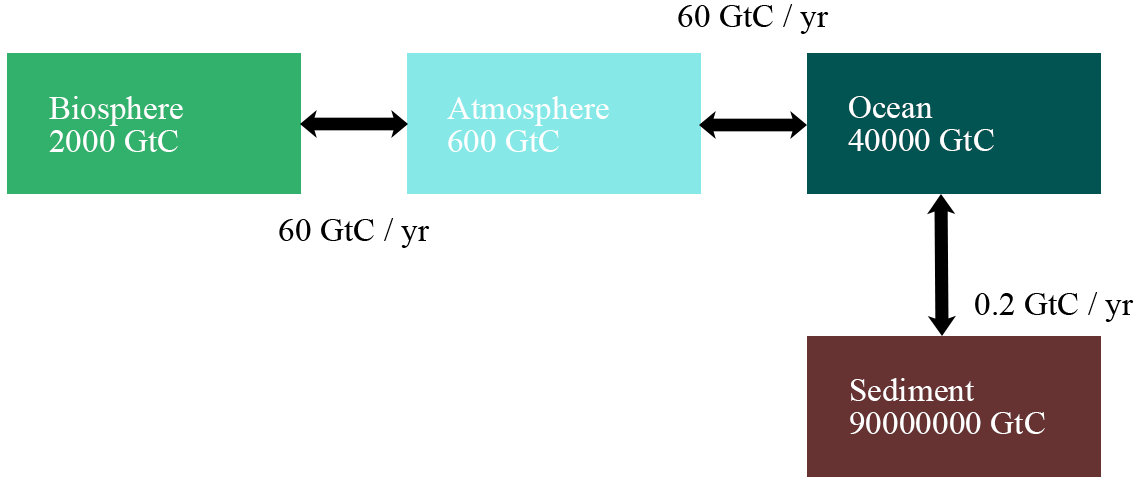
\includegraphics[scale = 1.1]{graphics/carboncycle.png}
\end{center}
\end{Exercise}

\begin{Exercise}
Daniel is drunk at a bar. He wants to go to the train station so that he can go home. However, since he is drunk, he loses his sense of direction, and will move randomly along the green edge (shown in the map below) once at a time. Assume that at any location, the chances of moving to all other neighboring locations are equal. Nevertheless, once he arrives at the train station, he will stop wandering and take the train. How many moves does it take on average for Daniel to reach the train station?
\begin{center}
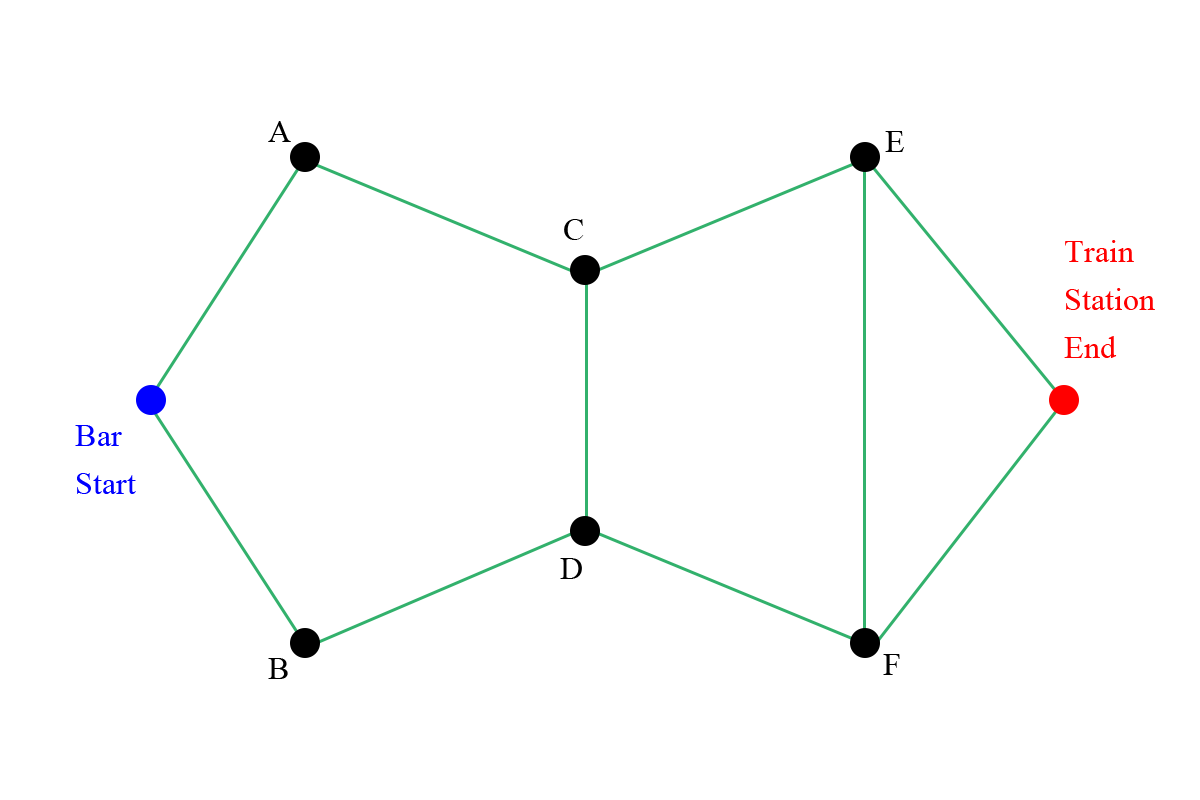
\includegraphics[scale = 0.3]{graphics/wander.png}
\end{center}
\end{Exercise}

\begin{Exercise}
Attempt \href{https://projecteuler.net/problem=84}{Project Euler Problem 84}, preferably with programming.
\end{Exercise}